\documentclass{article}
\usepackage[paperwidth=15cm,paperheight=9cm,margin=1cm]{geometry}
\usepackage{tikz}
\usetikzlibrary{arrows.meta}
\pagestyle{empty}
\definecolor{ink}{HTML}{344054}
\definecolor{blue}{HTML}{365F86}
\definecolor{clay}{HTML}{A45236}
\tikzset{every picture/.style={draw=ink,line width=.65pt,>=Stealth},every node/.style={text=ink}}
\begin{document}
\noindent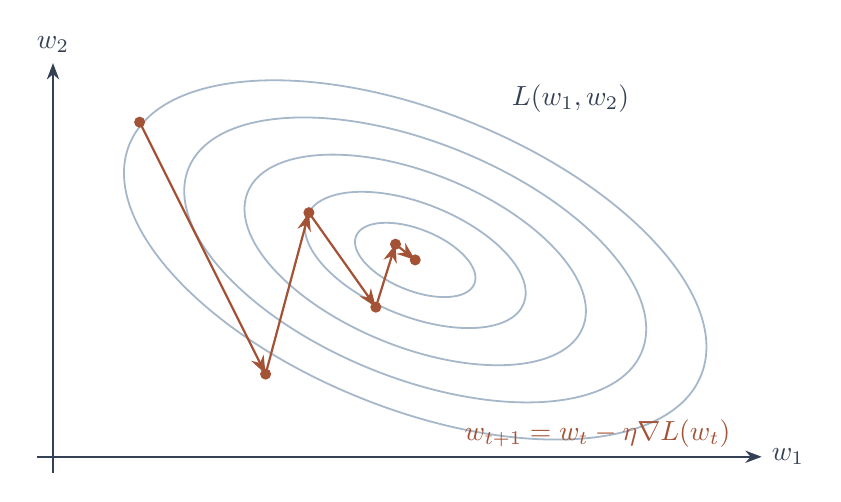
\begin{tikzpicture}[x=1cm,y=1cm]
\draw[->] (-.2,0)--(9,0) node[right] {$w_1$};
\draw[->] (0,-.2)--(0,5) node[above] {$w_2$};
\foreach \r in {0.6,1.1,1.7,2.3,2.9} {\draw[blue!45,rotate around={-22:(4.6,2.5)}] (4.6,2.5) ellipse ({1.35*\r} and {.65*\r});}
\draw[clay,thick,->] (1.1,4.25)--(2.7,1.05);
\draw[clay,thick,->] (2.7,1.05)--(3.25,3.1);
\draw[clay,thick,->] (3.25,3.1)--(4.1,1.9);
\draw[clay,thick,->] (4.1,1.9)--(4.35,2.7);
\draw[clay,thick,->] (4.35,2.7)--(4.6,2.5);
\foreach \x/\y in {1.1/4.25,2.7/1.05,3.25/3.1,4.1/1.9,4.35/2.7,4.6/2.5} {\fill[clay] (\x,\y) circle(2pt);}
\node[above right] at (5.7,4.25) {$L(w_1,w_2)$};
\node[below right,clay] at (5.1,.6) {$w_{t+1}=w_t-\eta\nabla L(w_t)$};
\end{tikzpicture}
\newpage
\noindent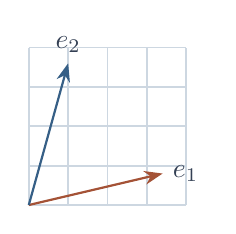
\begin{tikzpicture}
\draw[step=.5,blue!25] (0,0) grid (2,2);
\draw[->,thick,clay] (0,0)--(1.7,.4) node[right] {$e_1$};
\draw[->,thick,blue] (0,0)--(.5,1.8) node[above] {$e_2$};
\end{tikzpicture}
\newpage
\noindent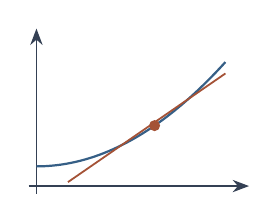
\begin{tikzpicture}
\draw[->] (-.1,0)--(2.7,0);\draw[->] (0,-.1)--(0,2);
\draw[blue,thick,domain=0:2.4,samples=40] plot (\x,{.23*(\x)^2+.25});
\draw[clay] (.4,.05)--(2.4,1.43);\fill[clay] (1.5,.7675) circle(2pt);
\end{tikzpicture}
\newpage
\noindent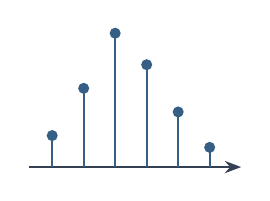
\begin{tikzpicture}
\draw[->] (0,0)--(2.7,0);
\foreach \x/\h in {.3/.4,.7/1,1.1/1.7,1.5/1.3,1.9/.7,2.3/.25} {\draw[blue,thick] (\x,0)--(\x,\h);\fill[blue] (\x,\h) circle(2pt);}
\end{tikzpicture}
\newpage
\noindent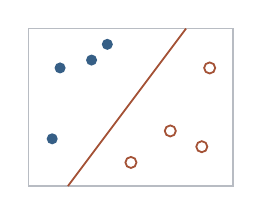
\begin{tikzpicture}
\draw[ink!35] (0,0) rectangle(2.6,2);
\draw[clay] (.5,0)--(2,2);
\foreach \x/\y in {.3/.6,.4/1.5,.8/1.6,1/1.8} {\fill[blue] (\x,\y) circle(2pt);}
\foreach \x/\y in {1.3/.3,1.8/.7,2.2/.5,2.3/1.5} {\draw[clay] (\x,\y) circle(2pt);}
\end{tikzpicture}
\newpage
\noindent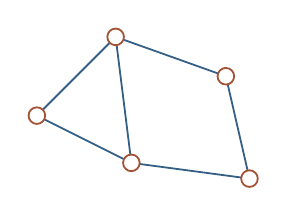
\begin{tikzpicture}
\foreach \a/\b in {1/2,1/3,2/3,2/4,3/5,4/5} {}
\coordinate (a) at (0,.8);\coordinate(b) at (1,1.8);\coordinate(c) at (1.2,.2);\coordinate(d) at (2.4,1.3);\coordinate(e) at (2.7,0);
\draw[blue] (a)--(b)--(c)--(a) (b)--(d)--(e)--(c);
\foreach \p in {a,b,c,d,e} {\filldraw[fill=white,draw=clay] (\p) circle(3pt);}
\end{tikzpicture}
\newpage
\noindent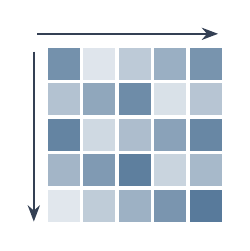
\begin{tikzpicture}[scale=.45]
\foreach \x in {0,...,4} {\foreach \y in {0,...,4} {\pgfmathtruncatemacro{\cellshade}{15+mod(\x*17+\y*31,70)}\fill[blue!\cellshade] (\x,\y) rectangle +(0.9,.9);}}
\draw[->] (-.3,5.3)--(4.8,5.3);\draw[->] (-.4,4.8)--(-.4,0);
\end{tikzpicture}
\end{document}
